\documentclass[tikz]{standalone}
\usetikzlibrary{automata,positioning}
\begin{document}

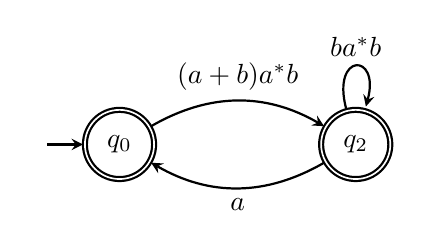
\begin{tikzpicture}[>=stealth,node distance=3cm,on grid,auto, thick, initial text=] 
  \node[state,initial,accepting] (q_0)   {$q_0$};
  \node[state,accepting]  (q_2) [right=3cm of q_0] {$q_2$};

  \path[->]     (q_0) edge [bend left] node {$(a+b)a^*b$} (q_2)
				(q_2) edge [bend left] node [below] {$a$} (q_0)
					edge [loop above] node [above] {$ba^*b$} (q_2);
                             
\end{tikzpicture}
\end{document}